\documentclass{article}
\usepackage{amsmath}
\usepackage{amssymb}
\usepackage{graphicx}
\usepackage{hyperref}
\usepackage[version=4]{mhchem}

\title{Example 4}
\date{}

\begin{document}
\maketitle

As shown in the figure, \(A B C D\) is a parallelogram. Draw a circle using \(A\) as the center and \(A B\) as the radius to meet \(B C\) at \(G, A D\) at \(F\), and the extension of \(B A\) at \(E\). Show that \(E F=F G\).

Solution:
Connect \(A G\). \(A B=A G . \angle B=\angle A G B=\alpha\).\\
Since \(B C / / A D, \angle B=\angle E A F=\alpha\) and \(\angle A G B=\angle G A F=\alpha\).\\
Thus \(\angle E A F=\angle G A F\) and they face the equal arcs or chords.\\
\centering
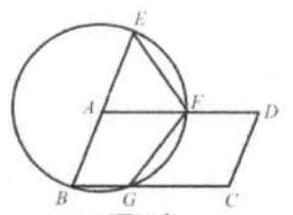
\includegraphics[width=\textwidth]{images/problem_image_1.jpg}

So \(E F=F G\).\\
\centering
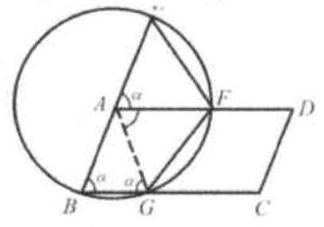
\includegraphics[width=\textwidth]{images/reasoning_image_1.jpg}


\end{document}
